\documentclass{standalone}
\usepackage{tikz}
\usetikzlibrary{patterns, positioning}
\usepackage[sfdefault]{ClearSans} %% option 'sfdefault' activates Clear Sans as the default text font
\usepackage[T1]{fontenc}

\begin{document}
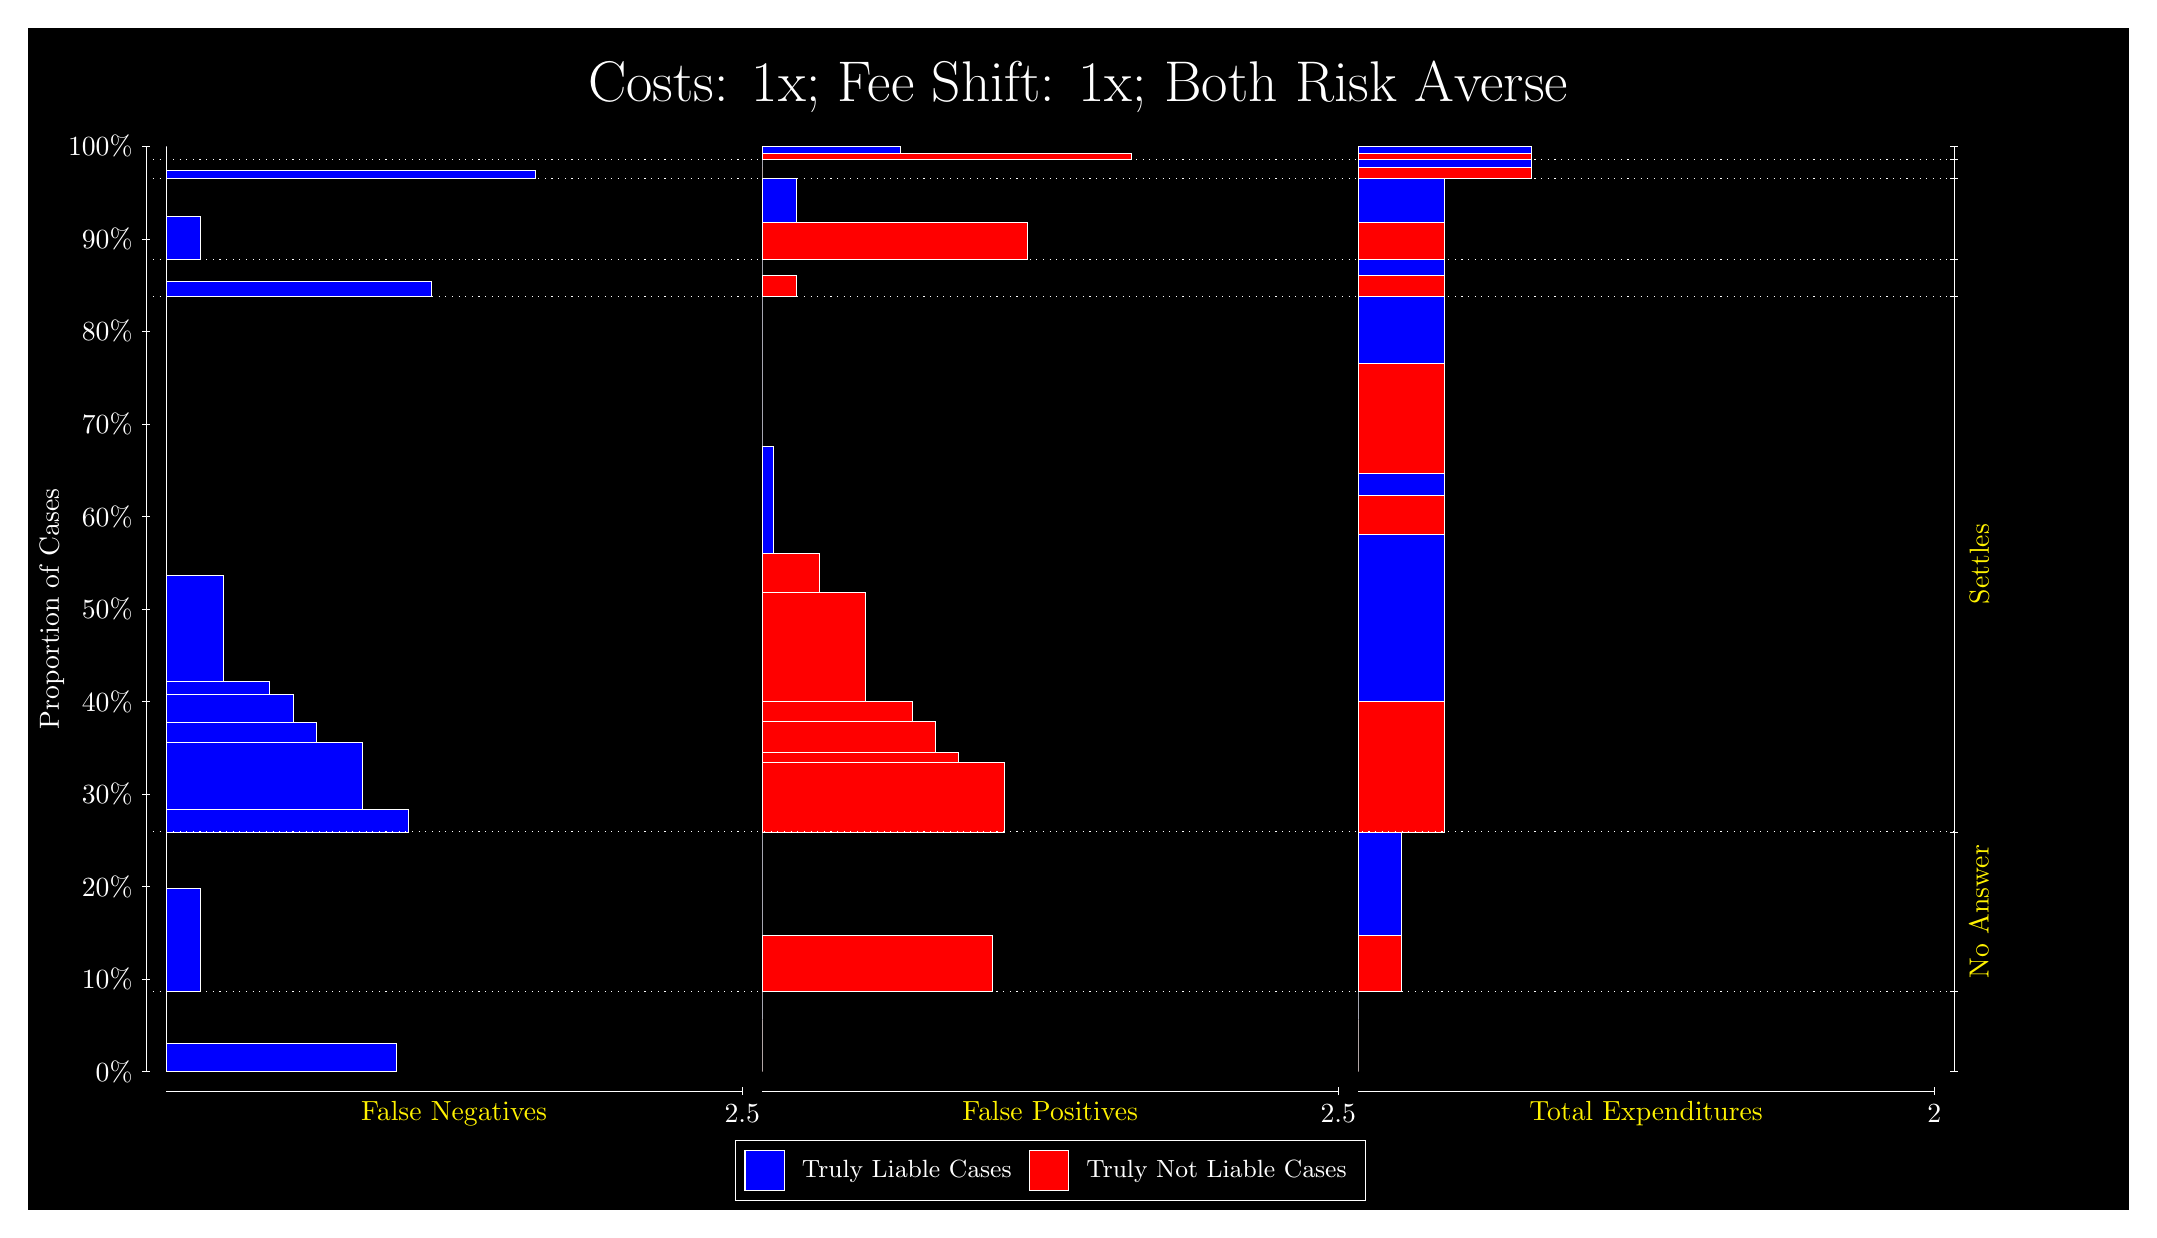
\begin{tikzpicture}
\draw[fill=black] (0,0) rectangle (26.667,15);
\draw[text=white] (0,13.5) rectangle (26.667,15) node[midway] {\huge Costs: 1x; Fee Shift: 1x; Both Risk Averse};
\draw[white, very thin] (1.5,1.75) -- (1.5,13.5);
\node[rotate=90, text=white, anchor=center] at (0.3, 7.625) {Proportion of Cases};
\draw[white, very thin] (1.45,1.75) -- (1.55,1.75);
\node[text=white, anchor=east] at (1.45, 1.75) {0\%};
\draw[white, very thin] (1.45,2.925) -- (1.55,2.925);
\node[text=white, anchor=east] at (1.45, 2.925) {10\%};
\draw[white, very thin] (1.45,4.1) -- (1.55,4.1);
\node[text=white, anchor=east] at (1.45, 4.1) {20\%};
\draw[white, very thin] (1.45,5.275) -- (1.55,5.275);
\node[text=white, anchor=east] at (1.45, 5.275) {30\%};
\draw[white, very thin] (1.45,6.45) -- (1.55,6.45);
\node[text=white, anchor=east] at (1.45, 6.45) {40\%};
\draw[white, very thin] (1.45,7.625) -- (1.55,7.625);
\node[text=white, anchor=east] at (1.45, 7.625) {50\%};
\draw[white, very thin] (1.45,8.8) -- (1.55,8.8);
\node[text=white, anchor=east] at (1.45, 8.8) {60\%};
\draw[white, very thin] (1.45,9.975) -- (1.55,9.975);
\node[text=white, anchor=east] at (1.45, 9.975) {70\%};
\draw[white, very thin] (1.45,11.15) -- (1.55,11.15);
\node[text=white, anchor=east] at (1.45, 11.15) {80\%};
\draw[white, very thin] (1.45,12.325) -- (1.55,12.325);
\node[text=white, anchor=east] at (1.45, 12.325) {90\%};
\draw[white, very thin] (1.45,13.5) -- (1.55,13.5);
\node[text=white, anchor=east] at (1.45, 13.5) {100\%};

\draw[white, very thin] (24.457,1.75) -- (24.457,13.5);
\draw[white, very thin] (24.407,1.75) -- (24.507,1.75);
\node[anchor=west] at (24.407, 1.75) {};
\draw[white, very thin] (24.407,2.7678) -- (24.507,2.7678);
\node[anchor=west] at (24.407, 2.7678) {};
\draw[white, very thin] (24.407,4.7945) -- (24.507,4.7945);
\node[anchor=west] at (24.407, 4.7945) {};
\draw[white, very thin] (24.407,11.595) -- (24.507,11.595);
\node[anchor=west] at (24.407, 11.595) {};
\draw[white, very thin] (24.407,12.061) -- (24.507,12.061);
\node[anchor=west] at (24.407, 12.061) {};
\draw[white, very thin] (24.407,13.097) -- (24.507,13.097);
\node[anchor=west] at (24.407, 13.097) {};
\draw[white, very thin] (24.407,13.337) -- (24.507,13.337);
\node[anchor=west] at (24.407, 13.337) {};
\draw[white, very thin] (24.407,13.5) -- (24.507,13.5);
\node[anchor=west] at (24.407, 13.5) {};

\draw[white, very thin, fill=blue] (1.75,1.75) rectangle (4.6775,2.1087);
\draw[white, very thin, fill=red] (1.75,2.1087) rectangle (1.75,2.7678);
\draw[white, very thin, fill=blue] (1.75,2.7678) rectangle (2.1891,4.0816);
\draw[white, very thin, fill=red] (1.75,4.0816) rectangle (1.75,4.7945);
\draw[white, very thin, fill=blue] (1.75,4.7945) rectangle (4.8239,5.085);
\draw[white, very thin, fill=blue] (1.75,5.085) rectangle (4.2384,5.9342);
\draw[white, very thin, fill=blue] (1.75,5.9342) rectangle (3.6529,6.1874);
\draw[white, very thin, fill=blue] (1.75,6.1874) rectangle (3.3602,6.5378);
\draw[white, very thin, fill=blue] (1.75,6.5378) rectangle (3.0674,6.7046);
\draw[white, very thin, fill=blue] (1.75,6.7046) rectangle (2.4819,8.0556);
\draw[white, very thin, fill=red] (1.75,8.0556) rectangle (1.75,11.595);
\draw[white, very thin, fill=blue] (1.75,11.595) rectangle (5.1167,11.792);
\draw[white, very thin, fill=red] (1.75,11.792) rectangle (1.75,12.061);
\draw[white, very thin, fill=blue] (1.75,12.061) rectangle (2.1891,12.617);
\draw[white, very thin, fill=red] (1.75,12.617) rectangle (1.75,13.097);
\draw[white, very thin, fill=blue] (1.75,13.097) rectangle (6.4341,13.199);
\draw[white, very thin, fill=red] (1.75,13.199) rectangle (1.75,13.337);
\draw[white, very thin, fill=red] (1.75,13.337) rectangle (1.75,13.414);
\draw[white, very thin, fill=blue] (1.75,13.414) rectangle (1.75,13.5);
\draw[white, very thin, fill=red] (9.3189,1.75) rectangle (9.3189,2.4091);
\draw[white, very thin, fill=blue] (9.3189,2.4091) rectangle (9.3189,2.7678);
\draw[white, very thin, fill=red] (9.3189,2.7678) rectangle (12.246,3.4807);
\draw[white, very thin, fill=blue] (9.3189,3.4807) rectangle (9.3189,4.7945);
\draw[white, very thin, fill=red] (9.3189,4.7945) rectangle (12.393,5.6713);
\draw[white, very thin, fill=red] (9.3189,5.6713) rectangle (11.807,5.8036);
\draw[white, very thin, fill=red] (9.3189,5.8036) rectangle (11.515,6.1961);
\draw[white, very thin, fill=red] (9.3189,6.1961) rectangle (11.222,6.4492);
\draw[white, very thin, fill=red] (9.3189,6.4492) rectangle (10.636,7.842);
\draw[white, very thin, fill=red] (9.3189,7.842) rectangle (10.051,8.3341);
\draw[white, very thin, fill=blue] (9.3189,8.3341) rectangle (9.4652,9.6851);
\draw[white, very thin, fill=blue] (9.3189,9.6851) rectangle (9.3189,11.595);
\draw[white, very thin, fill=red] (9.3189,11.595) rectangle (9.758,11.864);
\draw[white, very thin, fill=blue] (9.3189,11.864) rectangle (9.3189,12.061);
\draw[white, very thin, fill=red] (9.3189,12.061) rectangle (12.686,12.54);
\draw[white, very thin, fill=blue] (9.3189,12.54) rectangle (9.758,13.097);
\draw[white, very thin, fill=red] (9.3189,13.097) rectangle (9.3189,13.235);
\draw[white, very thin, fill=blue] (9.3189,13.235) rectangle (9.3189,13.337);
\draw[white, very thin, fill=red] (9.3189,13.337) rectangle (14.003,13.414);
\draw[white, very thin, fill=blue] (9.3189,13.414) rectangle (11.075,13.5);
\draw[white, very thin, fill=red] (16.888,1.75) rectangle (16.888,2.4091);
\draw[white, very thin, fill=blue] (16.888,2.4091) rectangle (16.888,2.7678);
\draw[white, very thin, fill=red] (16.888,2.7678) rectangle (17.437,3.4807);
\draw[white, very thin, fill=blue] (16.888,3.4807) rectangle (17.437,4.7945);
\draw[white, very thin, fill=red] (16.888,4.7945) rectangle (17.986,6.4492);
\draw[white, very thin, fill=blue] (16.888,6.4492) rectangle (17.986,8.5705);
\draw[white, very thin, fill=red] (16.888,8.5705) rectangle (17.986,9.0627);
\draw[white, very thin, fill=blue] (16.888,9.0627) rectangle (17.986,9.3532);
\draw[white, very thin, fill=red] (16.888,9.3532) rectangle (17.986,10.746);
\draw[white, very thin, fill=blue] (16.888,10.746) rectangle (17.986,11.595);
\draw[white, very thin, fill=red] (16.888,11.595) rectangle (17.986,11.864);
\draw[white, very thin, fill=blue] (16.888,11.864) rectangle (17.986,12.061);
\draw[white, very thin, fill=red] (16.888,12.061) rectangle (17.986,12.54);
\draw[white, very thin, fill=blue] (16.888,12.54) rectangle (17.986,13.097);
\draw[white, very thin, fill=red] (16.888,13.097) rectangle (19.083,13.235);
\draw[white, very thin, fill=blue] (16.888,13.235) rectangle (19.083,13.337);
\draw[white, very thin, fill=red] (16.888,13.337) rectangle (19.083,13.414);
\draw[white, very thin, fill=blue] (16.888,13.414) rectangle (19.083,13.5);
\draw[white, dotted] (1.5,2.7678) -- (24.457,2.7678);
\draw[white, dotted] (1.5,4.7945) -- (24.457,4.7945);
\draw[white, dotted] (1.5,11.595) -- (24.457,11.595);
\draw[white, dotted] (1.5,12.061) -- (24.457,12.061);
\draw[white, dotted] (1.5,13.097) -- (24.457,13.097);
\draw[white, dotted] (1.5,13.337) -- (24.457,13.337);
\draw[white, very thin] (1.75,1.5) -- (9.0689,1.5);
\node[text=yellow, anchor=north] at (5.4094, 1.5) {False Negatives};
\draw[white, very thin] (9.0689,1.45) -- (9.0689,1.55);
\node[text=white, anchor=north] at (9.0689, 1.45) {2.5};

\draw[white, very thin] (9.3189,1.5) -- (16.638,1.5);
\node[text=yellow, anchor=north] at (12.978, 1.5) {False Positives};
\draw[white, very thin] (16.638,1.45) -- (16.638,1.55);
\node[text=white, anchor=north] at (16.638, 1.45) {2.5};

\draw[white, very thin] (16.888,1.5) -- (24.207,1.5);
\node[text=yellow, anchor=north] at (20.547, 1.5) {Total Expenditures};
\draw[white, very thin] (24.207,1.45) -- (24.207,1.55);
\node[text=white, anchor=north] at (24.207, 1.45) {2};


\node[text=yellow, centered, rotate=90] at (24.777, 3.7812) {No Answer};
\node[text=yellow, centered, rotate=90] at (24.777, 8.1948) {Settles};





\draw (12.978300999999998,1.5) node[draw=none] (baseCoordinate) {};
\begin{scope}[align=center]
        \matrix[scale=0.5, draw=white, below=0.5cm of baseCoordinate, nodes={draw}, column sep=0.1cm]{
            \node[rectangle, draw, minimum width=0.5cm, minimum height=0.5cm, fill=blue] {}; &
            \node[draw=none, font=\small, text=white] (B) {Truly Liable Cases}; &
            \node[rectangle, draw, minimum width=0.5cm, minimum height=0.5cm, fill=red] {}; &
            \node[draw=none, font=\small, text=white] (B) {Truly Not Liable Cases}; \\
            };
\end{scope}

\end{tikzpicture}
\end{document}